\titre{}
\theme{}
\auteur{Nathan Scheinmann}
\niveau{}
\source{}
\type{serie}
\piments{1}
\pts{}
\annee{2526}

\contenu{
	\tcblower
On donne la fonction $f$ par son graphe.
\begin{center}
	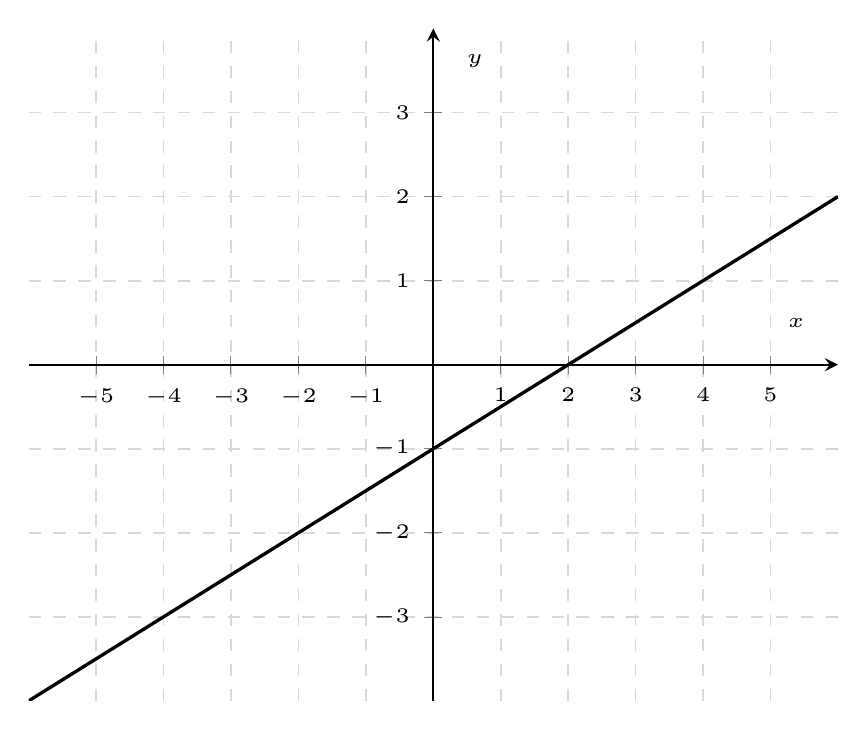
\begin{tikzpicture}[scale=1.5]
  \begin{axis}[
    axis lines=middle,
    xlabel={$x$}, ylabel={$y$},
    every axis x label/.style={at={(ticklabel* cs:0.92)}, anchor=west, yshift=10pt},
    every axis y label/.style={at={(ticklabel* cs:0.92)}, anchor=south, xshift=10pt},
    xmin=-6,   xmax=6,
    ymin=-4,   ymax=4,
    xtick={-5,-4,-3,-2,-1,0,1,2,3,4,5},
    ytick={-3,-2,-1,0,1,2,3},
    grid=both,
    grid style={dashed,gray!30},
    tick label style={font=\tiny},
    xlabel style={font=\tiny},
    ylabel style={font=\tiny}
  ]
    % branche pour x > 9
    \addplot[domain=-6:6, samples=200, thick]{0.5*x-1};
  \end{axis}
\end{tikzpicture}
\end{center}

Dessiner Le graphe des fonctions suivantes définies par :
\begin{tasks}(2)
  \task $g(x)=-f(x)$
  \task $h(x)=f(-x)$
  \task $i(x)=\begin{cases} f(x)& \text{si
                                  }f(x)\geq 0\\ -f(x)&\text{sinon}\end{cases}$
  \task $j(x)=\begin{cases} f(x)& \text{si
                                  }-f(x)\geq 0\\ f(x)&\text{sinon}\end{cases}$
                                \task $k(x)=f(x+2)$
                                \task $\ell(x)=f(x)-2$
                                \task $m(x)=f(x-1)+2$
                                \task $n(x)=2f(x)$
  \end{tasks}


}
\correction{
	\tcblower

}
